%%%%%%%%%%%%%%%%%%%%%%%%%%%%%%%%%%%%%%%%%
% CN2 Labreport template
%
% License:
% CC BY-NC-SA 3.0 (http://creativecommons.org/licenses/by-nc-sa/3.0/)
%
%%%%%%%%%%%%%%%%%%%%%%%%%%%%%%%%%%%%%%%%%

\documentclass[parskip=full]{scrartcl}

\usepackage{siunitx}  % Provides the \SI{}{} command for typesetting SI units
\usepackage{graphicx} % Required for the inclusion of images
\usepackage{booktabs} % nicer tables
\usepackage[noabbrev]{cleveref} % automatic references
\usepackage{listings} % typeset code
\usepackage[backend=biber]{biblatex}
\addbibresource{referenzen.bib}

\crefname{lstlisting}{listing}{listings} % for referencing code
\Crefname{lstlisting}{Listing}{Listings} % for referencing code

\usepackage[headsepline]{scrlayer-scrpage} % header
\ohead{Group 06} % right part of header
\ihead{Assignment 3} % left part of header

\lstset{basicstyle=\ttfamily} % monospaced font in listing



%----------------------------------------------------------------------------------------
%	DOCUMENT INFORMATION
%----------------------------------------------------------------------------------------

\begin{document}
\begin{titlepage}
    \centering
    \vspace*{2cm}
    {\Huge \textbf{Communication Networks 2}}\\
    SS 2021\\
    \vspace*{1cm}
    {\Large Assignment 3}
    \\\vspace*{3cm}
    {\Large \textbf{Group 06}}\\
    \vspace*{1cm}
    {\large 
        \begin{tabular}{l c c}
            Name & Mat.Nummer \\ \hline
            Paul Kloker & 12034928 \\
            Juan Aramis Oposich & 11701238
        \end{tabular}
    }
    \\\vspace*{7cm}
    \today
\end{titlepage}

%----------------------------------------------------------------------------------------
%	SECTION 1
%----------------------------------------------------------------------------------------
\section{Task description} \label{sec:task}

%----------------------------------------------------------------------------------------
%	SECTION 2
%----------------------------------------------------------------------------------------
\section{Procedure} \label{sec:procedure}
\subsection{Host discovery with nmap} \label{subsec:nmap}
\subsection{Ping measurements} \label{subsec:ping}
\subsection{Network topology}




\section{Data analysis and comparison} \label{sec:capture}


\begin{figure}[!ht]
	\centering % centering figure 
%	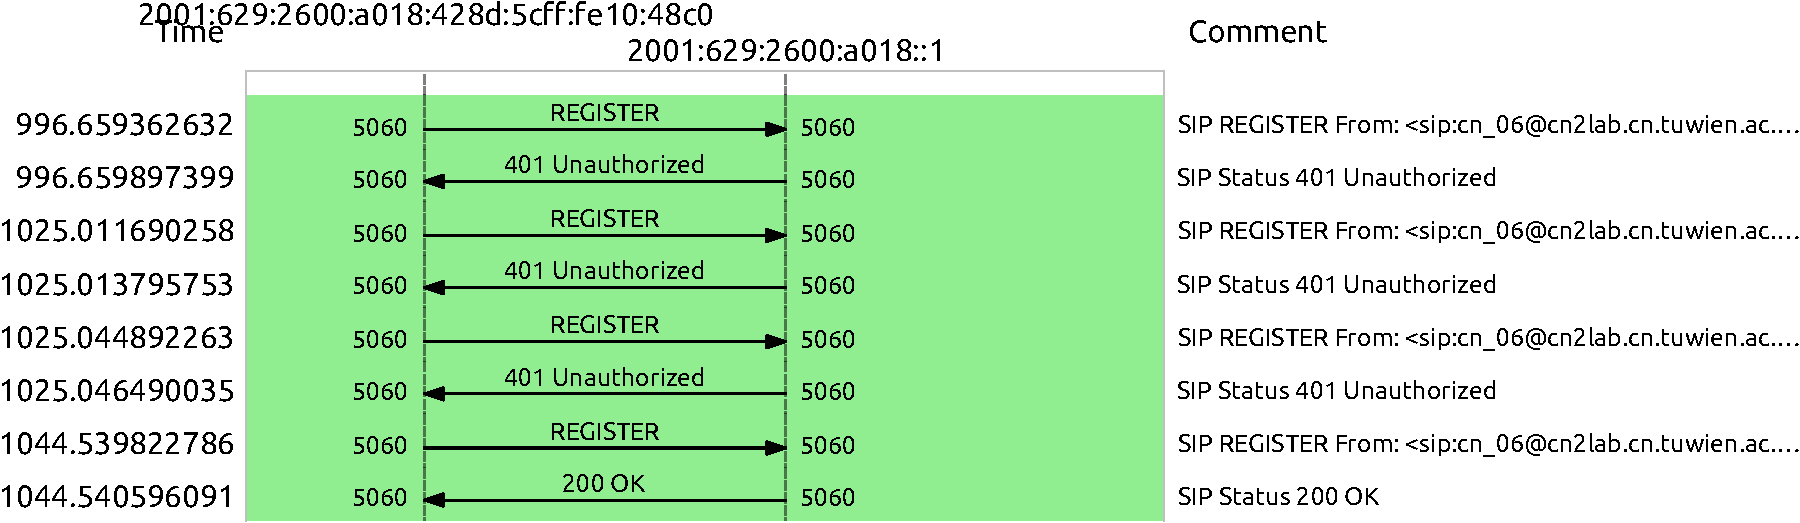
\includegraphics[width=\textwidth]{images/FlowSeqReg.pdf} % importing figure
	\caption{SIP registration flow} 
	\label{fig:SIP Registrar} % labeling to refer it inside the text
\end{figure}

\begin{table}[hb]
	\centering
	\begin{tabular}{|l|l|l|l|l|l|p{0.25\textwidth}|}
		\hline
		\textbf{No.} & \textbf{type} & \textbf{v. codec} &\textbf{v. score} & \textbf{a. codec} & \textbf{a. score} & \textbf{comment} \\ 
		\hline
		1 & landline & VP8 &5& OPUS &4&- \\
		\hline
		2 & satellite & VP8 &1 &  OPUS &3&no fluent video just single frames every view seconds\\
		\hline
	\end{tabular}
	\caption{Captured calls and quality rating (audio $\rightarrow$ a., video $\rightarrow$ v.)}
	\label{tab:capture}
\end{table}



%----------------------------------------------------------------------------------------
%	SECTION 3
%----------------------------------------------------------------------------------------
\newpage
\section{Conclusion}

%----------------------------------------------------------------------------------------
%	SECTION X
%---------------------------------------------------------------------------------------

\printbibliography

\end{document}
